\section{Stand der Technik}
\label{sec:stand_der_technik}

Die automatische Analyse von Straßenoberflächen entwickelt sich in den letzten Jahren. In diesem Kapitel werden die Grundlagen betrachtet, die für das Verständnis dieser Arbeit relevant sind. Die Analyse beginnt mit einer Betrachtung der Straßeninfrastruktur und der typischen Fahrbahnschäden. Anschließend werden die gängigen Klassifikationsstandards vorgestellt, um die Einordnung der Schäden zu ermöglichen. Schließlich erfolgt eine Einführung in die Computer Vision, welche die Grundlage für die KI-Modelle bildet, die in dieser Arbeit zum Einsatz kommen.

\subsection{Straßeninfrastruktur und typische Fahrbahnschäden}
\label{subsec:infrastruktur}

Für ein Verständnis, warum eine Straßenüberwachung notwendig ist, ist zunächst eine Betrachtung des Straßenaufbaus erforderlich. Eine Straße stellt ein komplexes Bauwerk dar, das aus mehreren Schichten mit jeweils spezifischen Aufgaben besteht.

Der Oberbau von Straßen besteht typischerweise aus einer Frostschutzschicht, einer oder mehreren Tragschichten sowie einer Asphalt- oder Betondeckschicht. Die einzelnen Schichten übernehmen unterschiedliche Aufgaben hinsichtlich Lastabtragung, Frostschutz und Oberflächenfunktion. Die Frostschutzschicht verhindert das Eindringen von Wasser und schützt vor Frostschäden. Die Tragschichten sorgen für die Lastverteilung und Stabilität der Straße, während die Deckschicht die direkte Kontaktfläche zum Verkehr bildet und für die Fahrqualität verantwortlich ist \cite{bmdv_asb_querschnitt_2024}.

Das Versagen einer dieser Schichten führt zur Entstehung von Schäden. Im Rahmen dieser Arbeit erfolgt eine Konzentration auf die Schadensarten, wie sie auch im Datensatz RDD2022 definiert sind \cite{rdd2022}:

\paragraph{Längsrisse, D00}
Diese Risse verlaufen parallel zur Fahrtrichtung. Die Entstehung erfolgt meistens in den Rollspuren schwerer Fahrzeuge. Mit der Zeit ermüdet das Material und bricht auf. Frühzeitig erkannte Längsrisse lassen sich mit speziellem Bitumen verfüllen, um das Eindringen von Wasser zu verhindern.

\paragraph{Querrisse, D10}
Diese Risse verlaufen quer zur Fahrbahn. Die Ursache liegt meist nicht in der Verkehrsbelastung, sondern in thermischen Einflüssen. Asphalt dehnt sich bei Hitze aus und zieht sich bei Kälte zusammen. Extreme Kälteperioden führen zu Spannungen im Material, die schließlich in thermischen Rissen resultieren.

\paragraph{Netzrisse, D20}
Netzrisse gelten als kritisch. Die Struktur ähnelt einem Spinnennetz oder der Haut eines Krokodils. Sie sind ein Indikator für eine Instabilität der tieferliegenden Schichten. In diesem Stadium ist eine einfache Reparatur meistens nicht mehr ausreichend, und es ist eine tiefergehende Sanierung erforderlich.

\paragraph{Schlaglöcher, D40}
Ein Schlagloch entsteht häufig als Folgeschaden von Rissen. In Risse eingedrungenes Wasser gefriert, dehnt sich aus und sprengt den Asphalt auf. Durch die mechanische Belastung nachfolgender Fahrzeuge brechen Materialstücke heraus. Schlaglöcher stellen ein Sicherheitsrisiko dar und können Fahrzeuge beschädigen.

\subsection{Computer Vision in der Infrastrukturüberwachung}
\label{subsec:cv_infrastruktur}

Die manuelle Analyse von Videoaufnahmen durch Experten ist zeitaufwendig, kostenintensiv und unterliegt subjektiven Einflüssen. Die Computer Vision ermöglicht die Automatisierung dieses Prozesses.

\paragraph{Der Sobel-Operator}
In der Computer Vision werden mathematische Filter zur Kantendetektion eingesetzt. Der Sobel-Operator sucht nach Helligkeitsunterschieden zwischen benachbarten Pixeln. Da Risse meist dunkler als die Umgebung sind, erzeugen sie eine detektierbare Helligkeits-Kante.

Der Operator nutzt hierzu kleine Matrizen, sogenannte Kernels, die über das Bild pixelweise geschoben werden. Dabei werden die Werte der Pixel mit den entsprechenden Werten des Kernels multipliziert und aufsummiert, um die Stärke der Kante zu bestimmen \cite[Kapitel 3.2]{szeliski2022computer}:
\begin{equation}
    G_x = \begin{bmatrix} -1 & 0 & +1 \\ -2 & 0 & +2 \\ -1 & 0 & +1 \end{bmatrix} * A, \quad G_y = \begin{bmatrix} +1 & +2 & +1 \\ 0 & 0 & 0 \\ -1 & -2 & -1 \end{bmatrix} * A
\end{equation}
Ein Nachteil dieser Methode liegt in der Fehleranfälligkeit gegenüber Schatten, dunklen Steinen oder Ölspuren, die ebenfalls Helligkeitskanten erzeugen und somit zu Fehlalarmen führen können. Zudem erfasst der Sobel-Operator nur lokale Informationen, was bei komplexen Rissstrukturen zu falschen Detektionen führen kann. Daher sind bessere Methoden erforderlich, um die Herausforderungen der realen Straßenbilder zu bewältigen.

\paragraph{Die Hough-Transformation}
Zur Identifikation gerader Linien aus einer Menge von Punkten findet die Hough-Transformation Anwendung. Die Beschreibung der Linien erfolgt mathematisch über Polarkoordinaten. Jeder Punkt im Bildraum wird in den Parameterraum transformiert, wobei die Beziehung zwischen den Koordinaten eines Punktes $(x, y)$ und den Parametern einer Linie $(r, \phi)$ durch die folgende Gleichung gegeben ist \cite[Kapitel 7.4.2]{szeliski2022computer}:
\begin{equation}
    r = x \cdot \cos(\phi) + y \cdot \sin(\phi)
\end{equation}
Obwohl dieser Ansatz theoretisch zur Detektion von Längs- oder Querrissen geeignet scheint, ist er für reale Rissstrukturen oft unpräzise. Reale Risse verlaufen meist unregelmäßig, verzweigt oder unterbrochen.

\subsection{Deep Learning für Schadensdetektion}
\label{subsec:deep_learning}

Eine Entwicklung stellt das Deep Learning dar. Hierbei werden keine manuellen Merkmale vorgegeben. Stattdessen lernt das Programm die relevanten Charakteristika eigenständig anhand einer großen Menge an Beispieldaten.

\paragraph{Convolutional Neural Networks (CNNs)}
CNNs bilden einen Standard für Bilderkennungsaufgaben. Die Architektur ist der Funktionsweise des menschlichen Auges nachempfunden und besteht aus mehreren sequenziellen Schichten \cite{oshea2015introduction}:
\begin{enumerate}
    \item Convolutional Layer: Hier werden Filterkerne gelernt, die sich während des Trainings an die Daten anpassen. Die unteren Schichten detektieren einfache Merkmale wie Kanten. Die höheren Schichten erfassen komplexere Strukturen, wie die Form eines Risses. Die Filter werden über das Bild geschoben, um die Merkmale zu extrahieren.
    \item Pooling Layer: Diese Schichten fassen Informationen zusammen. Wenn ein Riss in einem Bereich gefunden wurde, wird das Bild verkleinert, aber die Information über das Vorhandensein eines Schadens bleibt erhalten. Das macht das Modell schneller.
    \item Activation Layer, Aktivierung: Hier erfolgt die Entscheidung über die Relevanz von Informationen, beispielsweise durch die ReLU-Funktion, die negative Signale eliminiert:
    \begin{equation}
        f(x) = \max(0, x)
    \end{equation}
    \item Fully Connected Layer: Am Ende des Netzwerks werden alle extrahierten Merkmale kombiniert, um eine Klassifikationsentscheidung zu treffen.
\end{enumerate}

Ein limitierender Faktor bei CNNs ist das lokale Sichtfeld der Filter. Globale Zusammenhänge, wie der Verlauf eines langen Risses über das gesamte Bild, erfordern eine Informationsweitergabe über viele Schichten, was zu Detailverlusten führen kann. Zudem sind CNNs anfällig für Störfaktoren wie Schatten oder Verschmutzungen, da sie hauptsächlich auf lokale Merkmale reagieren. Daher ist die Suche nach Modellen, die globale Beziehungen besser erfassen können, ein wichtiger Schritt in der Weiterentwicklung der Schadensdetektion.

\subsection{Grundlagen der Transformer-Architektur}
\label{subsec:transformer_grundlagen}

Die Transformer-Architektur wird ursprünglich von Vaswani et al. \cite{vaswani2017attention_neurips} für Aufgaben der natürlichen Sprachverarbeitung eingeführt. Im Gegensatz zu rekurrenten neuronalen Netzen, die Sequenzen sequenziell verarbeiten, basiert der Transformer auf Aufmerksamkeitsmechanismen (Attention Mechanisms). Dies ermöglicht eine Parallelisierung während des Trainings und eine effektive Erfassung von globalen Abhängigkeiten in den Daten.

\paragraph{Der Self-Attention-Mechanismus}
Das Kernkonzept des Transformers ist die \emph{Scaled Dot-Product Attention}. Sie ermöglicht es dem Modell, für jedes Element einer Eingabesequenz zu berechnen, wie stark es sich auf alle anderen Elemente der Sequenz konzentrieren soll.

Jedes Eingabewort beziehungsweise Token wird in drei Vektoren projiziert: einen Query-Vektor (Abfrage) $q$, einen Key-Vektor (Schlüssel) $k$ und einen Value-Vektor (Wert) $v$. Diese Projektionen erfolgen über lernbare Gewichtsmatrizen $W^Q$, $W^K$ und $W^V$:
\begin{equation}
    q = x \cdot W^Q, \quad k = x \cdot W^K, \quad v = x \cdot W^V
\end{equation}
Führt man diese Vektoren für die gesamte Eingabesequenz als Zeilen in Matrizen $Q \in \mathbb{R}^{N \times d_k}$, $K \in \mathbb{R}^{N \times d_k}$ und $V \in \mathbb{R}^{N \times d_v}$ zusammen, wobei $N$ die Sequenzlänge und $d_k, d_v$ die Dimensionen der Projektionen bezeichnen, lässt sich die Aufmerksamkeit für die gesamte Sequenz wie folgt berechnen \cite{vaswani2017attention_neurips}:
\begin{equation}
    \text{Attention}(Q, K, V) = \text{softmax}\left(\frac{QK^T}{\sqrt{d_k}}\right)V
\end{equation}
Der Skalierungsfaktor $1/\sqrt{d_k}$ ist entscheidend, da bei großen Dimensionen $d_k$ das Skalarprodukt sehr große Werte annehmen kann. Dies führt zu extrem kleinen Gradienten nach der Softmax-Funktion, was das Training erschwert.

\paragraph{Multi-Head Attention}
Um dem Modell zu ermöglichen, Informationen aus verschiedenen Darstellungsunterräumen an unterschiedlichen Positionen gleichzeitig zu betrachten, wird die \emph{Multi-Head Attention} eingesetzt. Statt einer einzigen Aufmerksamkeitsfunktion werden $h$ unterschiedliche Projektionen der Queries, Keys und Values gelernt. Die Ergebnisse der einzelnen Köpfe werden konkateniert und durch eine weitere lineare Transformation geführt:
\begin{equation}
    \text{MultiHead}(Q, K, V) = \text{Concat}(\text{head}_1, \dots, \text{head}_h)W^O
\end{equation}
wobei $\text{head}_i = \text{Attention}(QW_i^Q, KW_i^K, VW_i^V)$ und $W^O$ eine weitere Gewichtsmatrix ist. Diese Struktur ermöglicht es dem Modell, verschiedene Aspekte der Daten gleichzeitig zu erfassen, was insbesondere bei komplexen Aufgaben wie der Schadensdetektion von Vorteil ist.

\paragraph{Der Transformer-Encoder-Block}
Ein Transformer-Encoder-Block besteht aus zwei Hauptkomponenten, der Multi-Head Self-Attention und einem positionsweisen Feed-Forward-Netzwerk. Um ein stabiles Training tiefer Netzwerke zu gewährleisten, werden um beide Komponenten Residualverbindungen gelegt, gefolgt von einer Normierungslayer. Abbildung \ref{fig:transformer_encoder_block} veranschaulicht diesen Aufbau grafisch.

\begin{figure}[H]
    \centering
    \begin{tikzpicture}[
        node distance=0.8cm and 1.2cm,
        block/.style={draw, rectangle, rounded corners=3pt, minimum width=4.5cm, minimum height=0.8cm, align=center, fill=blue!10, draw=blue!60!black, thick},
        mlp/.style={draw, rectangle, rounded corners=3pt, minimum width=4.5cm, minimum height=0.8cm, align=center, fill=red!10, draw=red!60!black, thick},
        norm/.style={draw, rectangle, rounded corners=3pt, minimum width=4.5cm, minimum height=0.8cm, align=center, fill=yellow!15, draw=yellow!60!black, thick},
        add/.style={draw, circle, minimum size=0.55cm, fill=gray!15, draw=gray!60!black, thick, inner sep=0pt},
        arrow/.style={->, >=latex, thick}
    ]
        % Nodes
        \node (in) {Eingabe $z_{l-1}$};
        \node (ln1) [norm, above=of in] {Layer Normalization (LN)};
        \node (mhsa) [block, above=of ln1] {Multi-Head Self-Attention (MHSA)};
        \node (add1) [add, above=of mhsa] {$+$};
        
        \node (ln2) [norm, above=of add1] {Layer Normalization (LN)};
        \node (mlp1) [mlp, above=of ln2] {Feed-Forward-Netzwerk (MLP)};
        \node (add2) [add, above=of mlp1] {$+$};
        \node (out) [above=of add2] {Ausgabe $z_l$};
        
        % Paths
        \draw [arrow] (in) -- (ln1);
        \draw [arrow] (ln1) -- (mhsa);
        \draw [arrow] (mhsa) -- (add1);
        \draw [arrow] (add1) -- (ln2);
        \draw [arrow] (ln2) -- (mlp1);
        \draw [arrow] (mlp1) -- (add2);
        \draw [arrow] (add2) -- (out);
        
        % Residuals
        \draw [arrow] (in.north) -- ++(-3.0,0) |- (add1.west) node[pos=0.25, left] {Residual};
        \draw [arrow] (add1.north) -- ++(-3.0,0) |- (add2.west) node[pos=0.25, left] {Residual};
        
    \end{tikzpicture}
    \caption{Schematische Darstellung eines standardmäßigen Transformer-Encoder-Blocks \cite{vaswani2017attention_neurips}.}
    \label{fig:transformer_encoder_block}
\end{figure}

\subsection{Der Übergang zur Computer Vision: Vision Transformer (ViT)}
\label{subsec:vision_transformer}

Der Transformer verarbeitet eindimensionale Sequenzen von Vektoren (z. B. Wort-Embeddings). Um diese Architektur auf zweidimensionale Bilddaten anzuwenden, stellt Dosovitskiy et al. \cite{vit2020} den \emph{Vision Transformer} (ViT) vor. Der Übergang von Pixeln zu Tokens erfordert folgende methodische Schritte:

\paragraph{Patch-Aufteilung und lineare Projektion (Patch Embedding)}
Ein Bild $x \in \mathbb{R}^{H \times W \times C}$ (mit Höhe $H$, Breite $W$ und Farbkanälen $C$) wird in eine Sequenz von quadratischen Bildausschnitten, sogenannten \emph{Patches}, der Größe $P \times P$ zerlegt. Die Anzahl der Patches beträgt:
\begin{equation}
    N = \frac{H \cdot W}{P^2}
\end{equation}
Jeder Patch $x_p^i \in \mathbb{R}^{P^2 \cdot C}$ wird flachgeklopft und über eine lernbare lineare Projektionsmatrix $E \in \mathbb{R}^{(P^2 \cdot C) \times D}$ in einen Vektor der Dimension $D$ transformiert. Diese Projektion entspricht einer Faltung mit einem Kernel der Größe $P \times P$ und einer Schrittweite (\emph{Stride}) $P$.

\paragraph{Klassifikationstoken und Positions-Embeddings}
Der Transformer-Encoder besitzt keine Informationen über die räumliche Anordnung der Patches, somit müssen Positionsinformationen hinzugefügt werden. Hierzu werden lernbare, eindimensionale Positions-Embeddings $E_{\text{pos}} \in \mathbb{R}^{(N+1) \times D}$ zu den Patch-Projektionen addiert. $D$ ist die Dimension der Token-Embeddings.

Zusätzlich wird ein lernbarer Klassifikations-Token  $x_{\text{class}} \in \mathbb{R}^{1 \times D}$ an den Anfang der Sequenz vorangestellt. Der Zustand dieses Tokens am Ausgang des Transformer-Encoders ist die zusammengefasste Information des gesamten Bildes und dient als Eingabe für den Klassifikationskopf. Die initiale Eingabesequenz $z_0$ lautet somit:
\begin{equation}
    z_0 = [x_{\text{class}}; x_p^1 E; x_p^2 E; \dots; x_p^N E] + E_{\text{pos}}
\end{equation}

\paragraph{Grenzen des Vision Transformers}
Vit weißt zwei Einschränkungen auf, die für die Anwendung in der Schadensdetektion relevant sind:
\begin{enumerate}
    \item Quadratische Rechenzeitkomplexität: Die Berechnung der Self-Attention vergleicht jeden Patch mit jedem anderen Patch. Dies führt bei $N$ Patches zu einer Komplexität von $\mathcal{O}(N^2 \cdot D)$. Für hochauflösende Bilder, wie sie in der Straßenerfassung notwendig sind, wird der Rechen- und Speicheraufwand hoch.
    \item Single-Scale: ViT erzeugt im Verlauf des Netzwerks eine konstante Tokenanzahl und Token-Dimension. Für dichte Aufgaben wie die Objekterkennung oder Segmentierung sind hierarchische Merkmalskarten von Vorteil, um sowohl globale als auch lokale Informationen zu erfassen. ViT bietet diese Möglichkeit nicht, was die Erkennung feiner Details wie Risse erschwert.
\end{enumerate}

\subsection{Swin Transformer: Lokale Fenster und Verschiebung}
\label{subsec:swin_transformer}

Zur Lösung der Effizienz- und Skalierungsprobleme des ViT führen Liu et al. \cite{swin2021} den \emph{Swin Transformer} (Shifted Window Transformer) ein. Dieser vereint die Vorteile von CNNs mit der Stärke von Transformern.

\paragraph{Hierarchische Merkmalskarten (Patch Merging)}
Der Swin Transformer baut eine hierarchische Repräsentation auf, die der Funktionsweise klassischer CNNs ähnelt. Zu Beginn des Netzwerks werden sehr kleine Patches verarbeitet. In tieferen Stufen führt das \emph{Patch Merging}-Modul jeweils benachbarte $2 \times 2$ Patch-Embeddings zusammen. Dies reduziert die Gesamtzahl der Tokens um den Faktor 4, was einer Reduzierung der räumlichen Auflösung um den Faktor 2 entspricht, während die Feature-Dimension nach einer linearen Transformation verdoppelt wird (von $D$ auf $2D$).

\paragraph{Fensterbasierte Aufmerksamkeit (Window-based MSA)}
Um das Komplexitätsproblem zu lösen, teilt der Swin Transformer das Bild in ein Raster aus nicht überlappenden Fenstern der Größe $M \times M$ Patches (typischerweise $M=7$) auf. Da die Aufmerksamkeit nur innerhalb eines Fensters berechnet wird, sinkt die Komplexität auf $\mathcal{O}(M^2 \cdot N)$. Da $M$ konstant ist, wächst der Rechenaufwand linear mit der Bildgröße, was die Verarbeitung hochauflösender Eingabebilder ermöglicht. Das wird durch \emph{Window-based Multi-Head Self-Attention (W-MSA)} realisiert, bei der die Aufmerksamkeit nur innerhalb der definierten Fenster berechnet wird.

\paragraph{Verschobene Fensteraufmerksamkeit (Shifted Window MSA)}
Da die Aufmerksamkeit bei der fensterbasierte Aufmerksamkeit auf lokale Fenster beschränkt ist, findet kein Informationsaustausch über die Fenstergrenzen hinweg statt. Um diese Einschränkung aufzuheben, nutzt der Swin Transformer in aufeinanderfolgenden Encoder-Blöcken eine verschobene Fensteraufteilung, \emph{Shifted Window Multi-Head Self-Attention (SW-MSA)}. Dabei wird die Fensterpartitionierung diagonal um $(\lfloor M/2 \rfloor, \lfloor M/2 \rfloor)$ Patches verschoben (siehe Abbildung \ref{fig:swin_shifted_windows}). Die neu entstandenen Fenster schneiden die alten Grenzen, was eine schrittweise Informationsübertragung über das gesamte Bild hinweg über mehrere Schichten ermöglicht.

\begin{figure}[H]
    \centering
    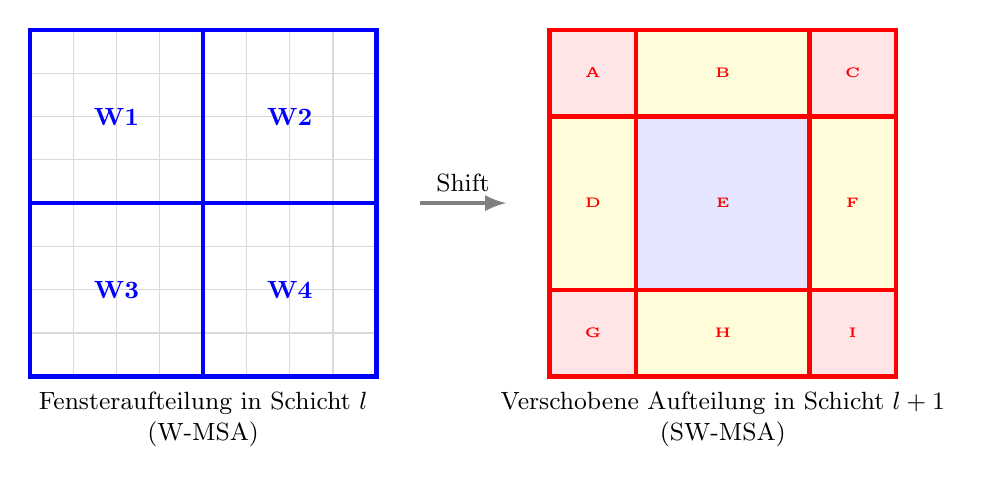
\begin{tikzpicture}[scale=0.55]
        % Left grid: W-MSA
        \begin{scope}[shift={(0,0)}]
            % Draw patches (8x8)
            \draw[gray!30, thin] (0,0) grid (8,8);
            % Draw windows (4x4)
            \draw[blue, ultra thick] (0,0) rectangle (4,4);
            \draw[blue, ultra thick] (4,0) rectangle (8,4);
            \draw[blue, ultra thick] (0,4) rectangle (4,8);
            \draw[blue, ultra thick] (4,4) rectangle (8,8);
            
            \node at (2,6) [blue, font=\small\bfseries] {W1};
            \node at (6,6) [blue, font=\small\bfseries] {W2};
            \node at (2,2) [blue, font=\small\bfseries] {W3};
            \node at (6,2) [blue, font=\small\bfseries] {W4};
            \node at (4,-1) [align=center, font=\small] {Fensteraufteilung in Schicht $l$\\ (W-MSA)};
        \end{scope}

        % Arrow in between
        \draw[->, >=latex, ultra thick, gray] (9,4) -- (11,4) node[above, midway, black, font=\small] {Shift};

        % Right grid: SW-MSA
        \begin{scope}[shift={(12,0)}]
            % Draw patches (8x8)
            \draw[gray!30, thin] (0,0) grid (8,8);
            
            % Shifted windows: shift is (2,2)
            % Draw rectangles for the 9 windows
            % Corner windows
            \draw[red, ultra thick, fill=red!10] (0,6) rectangle (2,8);
            \draw[red, ultra thick, fill=red!10] (6,6) rectangle (8,8);
            \draw[red, ultra thick, fill=red!10] (0,0) rectangle (2,2);
            \draw[red, ultra thick, fill=red!10] (6,0) rectangle (8,2);
            
            % Edge windows
            \draw[red, ultra thick, fill=yellow!15] (2,6) rectangle (6,8);
            \draw[red, ultra thick, fill=yellow!15] (0,2) rectangle (2,6);
            \draw[red, ultra thick, fill=yellow!15] (6,2) rectangle (8,6);
            \draw[red, ultra thick, fill=yellow!15] (2,0) rectangle (6,2);
            
            % Center window
            \draw[red, ultra thick, fill=blue!10] (2,2) rectangle (6,6);
            
            % Labels
            \node at (1,7) [red, font=\tiny\bfseries] {A};
            \node at (4,7) [red, font=\tiny\bfseries] {B};
            \node at (7,7) [red, font=\tiny\bfseries] {C};
            \node at (1,4) [red, font=\tiny\bfseries] {D};
            \node at (4,4) [red, font=\tiny\bfseries] {E};
            \node at (7,4) [red, font=\tiny\bfseries] {F};
            \node at (1,1) [red, font=\tiny\bfseries] {G};
            \node at (4,1) [red, font=\tiny\bfseries] {H};
            \node at (7,1) [red, font=\tiny\bfseries] {I};
            
            \node at (4,-1) [align=center, font=\small] {Verschobene Aufteilung in Schicht $l+1$\\ (SW-MSA)};
        \end{scope}
    \end{tikzpicture}
    \caption{Aufteilung eines Bildes in lokale Fenster bei W-MSA (links) und die verschobene Fensteraufteilung bei SW-MSA (rechts) mit einer Verschiebung um zwei Patches ($\lfloor M/2 \rfloor = 2$, für $M=4$). Durch die Verschiebung entstehen neue Fenstergrenzen, die den Informationsfluss zwischen benachbarten Fenstern ermöglichen (basierend auf \cite{swin2021}).}
    \label{fig:swin_shifted_windows}
\end{figure}

Um den Rechenaufwand auch bei verschobenen Fenstern minimal zu halten, wendet der Swin Transformer ein zyklisches Verschieben an. Bildbereiche, die durch die Verschiebung über den Rand hinausragen, werden virtuell auf die gegenüberliegende Seite des Bildes verschoben, um wieder vollständige Fenster zu bilden. Damit dabei keine fälschlichen Beziehungen zwischen eigentlich unzusammenhängenden Bildrändern berechnet werden, sorgt eine Maskierung im Aufmerksamkeitsmechanismus dafür, dass nur räumlich tatsächlich benachbarte Bereiche miteinander interagieren. Nach der Berechnung wird die ursprüngliche Bildreihenfolge wiederhergestellt.

\paragraph{Relative Positions-Bias (Relative Position Bias)}
Da die standardmäßige Self-Attention die Reihenfolge der Patches ignoriert, nutzt der Swin Transformer ein relatives Positionssystem anstelle absoluter Koordinaten. Hierbei wird ein gelernter relativer Positions-Bias $B$ direkt auf die berechnete Ähnlichkeitsmatrix addiert:
\begin{equation}
    \text{Attention}(Q, K, V) = \text{softmax}\left(\frac{QK^T}{\sqrt{d_k}} + B\right)V
\end{equation}
Anstatt jedem Patch eine feste Position im Gesamtbild zuzuweisen, beschreibt $B$ den relativen Abstand zwischen zwei Patches innerhalb eines Fensters. Da die Fenstergröße $M \times M$ klein und fest vorgegeben ist, ist die Anzahl möglicher relativer Positionen begrenzt, was die Lernbarkeit des Bias erleichtert. Dieser Ansatz ermöglicht es dem Modell, die räumlichen Beziehungen zwischen Patches besser zu erfassen.

\subsection{Cross-Entropy Loss (Kreuzentropie-Verlust)}
\label{subsec:cross_entropy}

Der Lernprozess aller betrachteten Deep-Learning-Modelle wird durch eine Fehlerfunktion gesteuert. Bei Klassifikationsaufgaben kommt standardmäßig der Cross-Entropy Loss zum Einsatz. Er misst die Abweichung zwischen der vorhergesagten Wahrscheinlichkeitsverteilung und der tatsächlichen Verteilung. Die Formel lautet:
\begin{equation}
    L = -\sum_{i=1}^{N_c} y_i \log(\hat{y}_i)
\end{equation}
Hierbei bezeichnet $N_c$ die Anzahl der Klassen, $y_i$ das tatsächliche Label (1 für die richtige Klasse, 0 für alle anderen) und $\hat{y}_i$ die vom Modell vorhergesagte Wahrscheinlichkeit für die Klasse $i$. Durch die Anpassung der Modellparameter während des Trainings über ein Gradientenabstiegsverfahren wird angestrebt, diesen Loss zu minimieren und somit die Klassifikationsgenauigkeit zu erhöhen \cite[Kapitel 5.7]{prince2023understanding}.

\subsection{Vergleich bestehender Systeme und Forschungsarbeiten}
\label{subsec:vergleich}

Existierende Systeme zur Straßenschadenerkennung verwenden häufig Laser-Scanner bzw. LiDAR-Systeme, da diese 3D-Informationen der Fahrbahnoberfläche liefern. Die Anschaffung und der Betrieb solcher Systeme sind jedoch mit hohen Kosten verbunden. Kamerabasierte Systeme stellen eine kostengünstigere Alternative dar, ihre Leistungsfähigkeit kann jedoch durch ungünstige Beleuchtungs- und Witterungsbedingungen beeinträchtigt werden \cite{hamaguchi2018development}.

Aktuelle Forschungsarbeiten belegen das Potenzial von Transformer-Modellen zur Überwindung dieser Einschränkungen. Die vorliegende Arbeit, HSP 2, baut auf diesen Erkenntnissen auf und untersucht Strategien zur Klassifikationsgenauigkeit für den Einsatz in Sanierungsplanungen. Eine Rolle spielt hierbei das Transfer Learning, bei dem vortrainierte Modelle auf die Anforderungen der Straßenschadenserkennung angepasst werden \cite[Kapitel 4]{amaratunga2023}.
